\section{3928 - Ballroom Lights}
\textbf{Problema:}
Dada una vista superior de una habitaci'on rectangular en la que hay una serie de 
luces (fuentes puntuales de luz) y de columnas (cilindros), determinar la porci'on
del per'imetro de la habitaci'on que se encuentra iluminada por las luces.

\subsection{Resoluci\'on}

La soluci'on del problema consiste en calcular los efectos individuales de cada
luz sobre cada columna considerando una 'unica pared, y luego combinarlos de manera 
de obtener el resultado total. Para esto, se considera en primer lugar como se 
resuelve el caso particular conociendo la ubicaci'on de ambas dentro de la habitaci'on, las
dimensiones de la misma y el radio de la columna.

\begin{figure}[H]
\centering
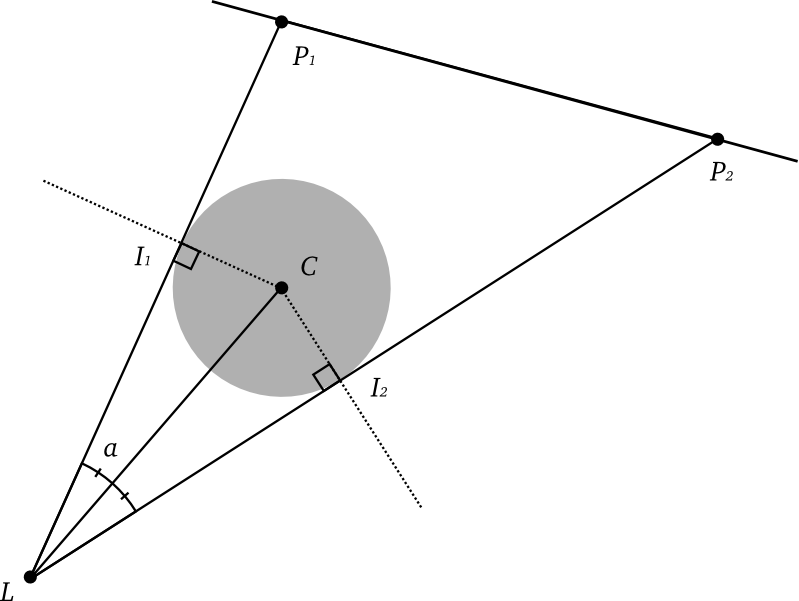
\includegraphics[width=12cm]{./figuras/ballroom.png}
\caption{Esquema del caso particular (1 columna, 1 luz, 1 pared)}
\end{figure}

Esta situaci'on se resuelve con trigonometr'ia simple: conociendo el radio de la
columna ($|I_{1}C|$) y la distancia entre la luz y el centro de la misma ($|LC|$),
podemos calcular el 'angulo $a$:

$$a = sin^{-1}\frac{|I_{1}C|}{|LC|}$$

Con el 'angulo $a$ resulta sencillo construir las intersecciones con la pared posterior.
Es importante tener en cuenta el caso en que dicha intersecci'on no existe (estamos
tratando con una semirecta de origen $L$), o se encuentra fuera del segmento que
corresponde a la pared.

Finalmente, se calcula el largo del segmento oscurecido por la columna que cae dentro
de la pared. Con este dato, el algoritmo completo es el siguiente:

\begin{algorithm}[H]
\begin{algorithmic}
\caption{Calcular la longitud del perímetro iluminado}
\FOR{cada pared}
  \FOR{cada luz}
    \FOR{cada columna}
        \STATE obtener la zona oscurecida de esta terna
    \ENDFOR
    \STATE unir todas las sombras de esta luz
    \STATE invertir las sombras para obtener las zonas iluminadas de esta luz
  \ENDFOR
  \STATE unir todas las zonas iluminadas por cada luz
  \STATE calcular la longitud iluminada en esta pared
\ENDFOR
\STATE devolver la suma de las longitudes iluminadas sobre cada pared
\end{algorithmic}
\end{algorithm}

\subsubsection{Implementaci'on}

La implementaci'on no tiene mayores particularidades. Nos encontramos con
un problema de error num'erico producto de la utilizaci�n valores obtenidos
con las funciones trigonom'etricas. Lo resolvimos utilizando \textbf{long double}
para aumentar la precisi'on de las operaciones.

Muchos de los datos utilizados en el programa son conjuntos de intervalos
que representan una porci'on (eventualmente discontinua) de los segmentos
que corresponden a las paredes. Estos conjuntos se implementaron sobre secuencias.


\subsubsection{Complejidad}

Llamaremos $C$ a la cantidad de columnas y $L$ a la cantidad de luces.

Las operaciones utilizadas por el algoritmo son:
\begin{itemize}
\item \textbf{B'usqueda de puntos de intersecci'on}, que se hace en tiempo constante en el modelo uniforme.
\item \textbf{Uni'on de conjuntos de intervalos}, que se hace en $O(n log(n))$ orden'andolos primero.
\item \textbf{Inversi'on de conjuntos de intervalos}, que se hace en $O(n)$ puesto que ya est'an ordenados.
\item \textbf{C'alculo de la longitud cubierta por el conjunto}, que se hace en $O(n)$ puesto que ya est'an ordenados.
\end{itemize}

Sabemos adem'as que cada columna tiene a lo sumo una sombra sobre cada pared. Por lo tanto,
unir todas las sombras de una luz se hace en $O(C log(C))$. En peor caso, el conjunto
resultante tiene $C$ elementos, lo que corresponde al caso en que todas las sombras
de las columnas son disjuntas.

La inversi'on se hace entonces en $O(C)$. Para los 'ultimos pasos del ciclo sobre las luces,
se unen las sombras de cada una de ellas. Dado que en peor caso tenemos $L * C$ intervalos
a unir, la uni'on resulta en un costo de $O(LC log(LC))$, seguido del c'alculo de la
longitud en tiempo lineal con un costo de $O(LC)$ dado que tras la uni'on el conjunto
de intervalos se encuentra ordenado.

Estas operaciones se hacen para cada pared, con un total de 4 que no afecta la complejidad
puesto que es constante. Finalmente, el algoritmo tiene un costo de $O(LC log(LC))$, que es
polinomial en el tama~no de la entrada puesto que la misma tiene tama\~no $O(L+C+t)$ (con
$t=log_2(max(ancho, alto))$).

\subsection{Implementaci�n}

\noindent
\ttfamily
\shorthandoff{"}\\
\hlstd{}\hlline{\ 1\ }\hldir{\#include\ $<$iostream$>$}\\
\hlline{\ 2\ }\hlstd{}\hldir{\#include\ $<$cmath$>$}\\
\hlline{\ 3\ }\hlstd{}\hldir{\#include\ $<$cstdio$>$}\\
\hlline{\ 4\ }\hlstd{}\hldir{\#include\ $<$list$>$}\\
\hlline{\ 5\ }\hlstd{}\hldir{\#include\ $<$utility$>$}\\
\hlline{\ 6\ }\hlstd{}\hldir{\#include\ $<$cstdlib$>$}\\
\hlline{\ 7\ }\hlstd{}\hldir{\#include\ $<$cassert$>$}\\
\hlline{\ 8\ }\hlstd{}\hldir{\#include\ $<$complex$>$}\\
\hlline{\ 9\ }\hlstd{}\\
\hlline{10\ }\hldir{\#define\ forn(i,\ n)\ for\ (int\ i\ =\ 0;\ i\ $<$\ (n);\ i++)}\\
\hlline{11\ }\hlstd{}\hldir{\#define\ TOLERANCIA\ 1e{-}8}\\
\hlline{12\ }\hlstd{}\\
\hlline{13\ }\hlkwa{using\ namespace\ }\hlstd{std}\hlsym{;}\\
\hlline{14\ }\hlstd{}\\
\hlline{15\ }\hlkwb{struct\ }\hlstd{MaybeDouble\ }\hlsym{\{}\\
\hlline{16\ }\hlstd{}\hlstd{\ \ \ \ }\hlstd{}\hlkwb{long\ double\ }\hlstd{valor}\hlsym{;}\\
\hlline{17\ }\hlstd{}\hlstd{\ \ \ \ }\hlstd{}\hlkwb{bool\ }\hlstd{valido}\hlsym{;}\\
\hlline{18\ }\hlstd{\\
\hlline{19\ }}\hlstd{\ \ \ \ }\hlstd{}\hlkwd{MaybeDouble}\hlstd{}\hlsym{(}\hlstd{}\hlkwb{long\ double\ }\hlstd{v}\hlsym{,\ }\hlstd{}\hlkwb{bool\ }\hlstd{b}\hlsym{):\ }\hlstd{}\hlkwd{valor}\hlstd{}\hlsym{(}\hlstd{v}\hlsym{),\ }\hlstd{}\hlkwd{valido}\hlstd{}\hlsym{(}\hlstd{b}\hlsym{)\ \{\};}\\
\hlline{20\ }\hlstd{}\hlsym{\};}\\
\hlline{21\ }\hlstd{}\\
\hlline{22\ }\hlkwb{struct\ }\hlstd{Vector\ }\hlsym{\{}\\
\hlline{23\ }\hlstd{}\hlstd{\ \ \ \ }\hlstd{}\hlkwb{long\ double\ }\hlstd{x}\hlsym{;}\\
\hlline{24\ }\hlstd{}\hlstd{\ \ \ \ }\hlstd{}\hlkwb{long\ double\ }\hlstd{y}\hlsym{;}\\
\hlline{25\ }\hlstd{\\
\hlline{26\ }}\hlstd{\ \ \ \ }\hlstd{}\hlkwd{Vector}\hlstd{}\hlsym{(}\hlstd{}\hlkwb{long\ double\ }\hlstd{xi}\hlsym{,\ }\hlstd{}\hlkwb{long\ double\ }\hlstd{yi}\hlsym{):\ }\hlstd{}\hlkwd{x}\hlstd{}\hlsym{(}\hlstd{xi}\hlsym{),\ }\hlstd{}\hlkwd{y}\hlstd{}\hlsym{(}\hlstd{yi}\hlsym{)\ \{\};}\\
\hlline{27\ }\hlstd{\\
\hlline{28\ }}\hlstd{\ \ \ \ }\hlstd{}\hlkwb{long\ double\ }\hlstd{}\hlkwd{norma}\hlstd{}\hlsym{()}\hlstd{\ \ }\hlsym{\{}\\
\hlline{29\ }\hlstd{}\hlstd{\ \ \ \ \ \ \ \ }\hlstd{}\hlkwa{return\ }\hlstd{}\hlkwd{hypot}\hlstd{}\hlsym{(}\hlstd{x}\hlsym{,\ }\hlstd{y}\hlsym{);}\\
\hlline{30\ }\hlstd{}\hlstd{\ \ \ \ }\hlstd{}\hlsym{\}}\\
\hlline{31\ }\hlstd{\\
\hlline{32\ }}\hlstd{\ \ \ \ }\hlstd{}\hlkwb{long\ double\ }\hlstd{}\hlkwd{angulo}\hlstd{}\hlsym{()\ \{}\\
\hlline{33\ }\hlstd{}\hlstd{\ \ \ \ \ \ \ \ }\hlstd{}\hlkwa{return\ }\hlstd{}\hlkwd{atan2}\hlstd{}\hlsym{(}\hlstd{y}\hlsym{,\ }\hlstd{x}\hlsym{);}\\
\hlline{34\ }\hlstd{}\hlstd{\ \ \ \ }\hlstd{}\hlsym{\}}\\
\hlline{35\ }\hlstd{}\\
\hlline{36\ }\hlsym{\};}\\
\hlline{37\ }\hlstd{}\\
\hlline{38\ }\hlkwb{struct\ }\hlstd{Columna\ }\hlsym{\{}\\
\hlline{39\ }\hlstd{}\hlstd{\ \ \ \ }\hlstd{Vector\ posicion}\hlsym{;}\\
\hlline{40\ }\hlstd{}\hlstd{\ \ \ \ }\hlstd{}\hlkwb{long\ double\ }\hlstd{radio}\hlsym{;}\\
\hlline{41\ }\hlstd{\\
\hlline{42\ }}\hlstd{\ \ \ \ }\hlstd{}\hlkwd{Columna}\hlstd{}\hlsym{(}\hlstd{}\hlkwb{long\ double\ }\hlstd{x}\hlsym{,\ }\hlstd{}\hlkwb{long\ double\ }\hlstd{y}\hlsym{,\ }\hlstd{}\hlkwb{long\ double\ }\hlstd{r}\hlsym{)\ :\ }\hlstd{}\hlkwd{posicion}\hlstd{}\hlsym{(}\hlstd{x}\hlsym{,}\hlstd{y}\hlsym{),\ }\hlstd{}\hlkwd{radio}\hlstd{}\hlsym{(}\hlstd{r}\hlsym{)\ \{\};}\\
\hlline{43\ }\hlstd{}\hlsym{\};}\\
\hlline{44\ }\hlstd{}\\
\hlline{45\ }\hlkwc{typedef\ }\hlstd{Vector\ Lampara}\hlsym{;}\\
\hlline{46\ }\hlstd{}\hlkwc{typedef\ }\hlstd{pair}\hlsym{$<$}\hlstd{}\hlkwb{long\ double}\hlstd{}\hlsym{,\ }\hlstd{}\hlkwb{long\ double}\hlstd{}\hlsym{$>$\ }\hlstd{Intervalo}\hlsym{;}\\
\hlline{47\ }\hlstd{}\hlkwc{typedef\ }\hlstd{pair}\hlsym{$<$}\hlstd{Vector}\hlsym{,\ }\hlstd{Vector}\hlsym{$>$\ }\hlstd{Segmento}\hlsym{;}\\
\hlline{48\ }\hlstd{}\\
\hlline{49\ }\\
\hlline{50\ }\hlkwc{inline\ }\hlstd{}\hlkwb{long\ double\ }\hlstd{}\hlkwd{largo}\hlstd{}\hlsym{(}\hlstd{}\hlkwb{const\ }\hlstd{Segmento}\hlsym{\&\ }\hlstd{s}\hlsym{)\ \{}\\
\hlline{51\ }\hlstd{}\hlstd{\ \ \ \ }\hlstd{}\hlkwa{return\ }\hlstd{}\hlkwd{Vector}\hlstd{}\hlsym{(}\hlstd{s}\hlsym{.}\hlstd{second}\hlsym{.}\hlstd{x\ }\hlsym{{-}\ }\hlstd{s}\hlsym{.}\hlstd{first}\hlsym{.}\hlstd{x}\hlsym{,\ }\hlstd{s}\hlsym{.}\hlstd{second}\hlsym{.}\hlstd{y\ }\hlsym{{-}\ }\hlstd{s}\hlsym{.}\hlstd{first}\hlsym{.}\hlstd{y}\hlsym{).}\hlstd{}\hlkwd{norma}\hlstd{}\hlsym{();}\\
\hlline{52\ }\hlstd{}\hlsym{\}}\\
\hlline{53\ }\hlstd{}\\
\hlline{54\ }\hlkwc{inline\ }\hlstd{}\hlkwb{long\ double\ }\hlstd{}\hlkwd{largo}\hlstd{}\hlsym{(}\hlstd{}\hlkwb{const\ }\hlstd{Intervalo}\hlsym{\&\ }\hlstd{i}\hlsym{)\ \{}\\
\hlline{55\ }\hlstd{}\hlstd{\ \ \ \ }\hlstd{}\hlkwd{assert}\hlstd{}\hlsym{(}\hlstd{i}\hlsym{.}\hlstd{first\ }\hlsym{$<$=\ }\hlstd{i}\hlsym{.}\hlstd{second}\hlsym{);}\\
\hlline{56\ }\hlstd{}\hlstd{\ \ \ \ }\hlstd{}\hlkwa{return\ }\hlstd{i}\hlsym{.}\hlstd{second\ }\hlsym{{-}\ }\hlstd{i}\hlsym{.}\hlstd{first}\hlsym{;}\\
\hlline{57\ }\hlstd{}\hlsym{\}}\\
\hlline{58\ }\hlstd{\\
\hlline{59\ }\\
\hlline{60\ }MaybeDouble\ }\hlkwd{intersect\textunderscore segments}\hlstd{}\hlsym{(}\hlstd{}\hlkwb{const\ }\hlstd{Segmento}\hlsym{\&\ }\hlstd{s1}\hlsym{,\ }\hlstd{}\hlkwb{const\ }\hlstd{Segmento}\hlsym{\&\ }\hlstd{s2}\hlsym{)\ \{}\\
\hlline{61\ }\hlstd{}\hlstd{\ \ \ \ }\hlstd{Vector\ p1\ }\hlsym{=\ }\hlstd{s1}\hlsym{.}\hlstd{first}\hlsym{;}\\
\hlline{62\ }\hlstd{}\hlstd{\ \ \ \ }\hlstd{Vector\ p2\ }\hlsym{=\ }\hlstd{s1}\hlsym{.}\hlstd{second}\hlsym{;}\\
\hlline{63\ }\hlstd{}\hlstd{\ \ \ \ }\hlstd{Vector\ p3\ }\hlsym{=\ }\hlstd{s2}\hlsym{.}\hlstd{first}\hlsym{;}\\
\hlline{64\ }\hlstd{}\hlstd{\ \ \ \ }\hlstd{Vector\ p4\ }\hlsym{=\ }\hlstd{s2}\hlsym{.}\hlstd{second}\hlsym{;}\\
\hlline{65\ }\hlstd{\\
\hlline{66\ }}\hlstd{\ \ \ \ }\hlstd{}\hlkwb{long\ double\ }\hlstd{den\ }\hlsym{=\ (}\hlstd{p4}\hlsym{.}\hlstd{y}\hlsym{{-}}\hlstd{p3}\hlsym{.}\hlstd{y}\hlsym{){*}(}\hlstd{p2}\hlsym{.}\hlstd{x}\hlsym{{-}}\hlstd{p1}\hlsym{.}\hlstd{x}\hlsym{)\ {-}\ (}\hlstd{p4}\hlsym{.}\hlstd{x}\hlsym{{-}}\hlstd{p3}\hlsym{.}\hlstd{x}\hlsym{){*}(}\hlstd{p2}\hlsym{.}\hlstd{y}\hlsym{{-}}\hlstd{p1}\hlsym{.}\hlstd{y}\hlsym{);}\\
\hlline{67\ }\hlstd{\\
\hlline{68\ }}\hlstd{\ \ \ \ }\hlstd{}\hlkwb{long\ double\ }\hlstd{ua\textunderscore num\ }\hlsym{=\ (}\hlstd{p4}\hlsym{.}\hlstd{x}\hlsym{{-}}\hlstd{p3}\hlsym{.}\hlstd{x}\hlsym{){*}(}\hlstd{p1}\hlsym{.}\hlstd{y}\hlsym{{-}}\hlstd{p3}\hlsym{.}\hlstd{y}\hlsym{)\ {-}\ (}\hlstd{p4}\hlsym{.}\hlstd{y}\hlsym{{-}}\hlstd{p3}\hlsym{.}\hlstd{y}\hlsym{){*}(}\hlstd{p1}\hlsym{.}\hlstd{x}\hlsym{{-}}\hlstd{p3}\hlsym{.}\hlstd{x}\hlsym{);}\\
\hlline{69\ }\hlstd{}\hlstd{\ \ \ \ }\hlstd{}\hlkwb{long\ double\ }\hlstd{ub\textunderscore num\ }\hlsym{=\ (}\hlstd{p2}\hlsym{.}\hlstd{x}\hlsym{{-}}\hlstd{p1}\hlsym{.}\hlstd{x}\hlsym{){*}(}\hlstd{p1}\hlsym{.}\hlstd{y}\hlsym{{-}}\hlstd{p3}\hlsym{.}\hlstd{y}\hlsym{)\ {-}\ (}\hlstd{p2}\hlsym{.}\hlstd{y}\hlsym{{-}}\hlstd{p1}\hlsym{.}\hlstd{y}\hlsym{){*}(}\hlstd{p1}\hlsym{.}\hlstd{x}\hlsym{{-}}\hlstd{p3}\hlsym{.}\hlstd{x}\hlsym{);}\\
\hlline{70\ }\hlstd{\\
\hlline{71\ }}\hlstd{\ \ \ \ }\hlstd{}\hlkwa{if\ }\hlstd{}\hlsym{(}\hlstd{}\hlkwd{fabs}\hlstd{}\hlsym{(}\hlstd{den}\hlsym{)\ $<$\ }\hlstd{TOLERANCIA}\hlsym{)\ \{}\\
\hlline{72\ }\hlstd{}\hlstd{\ \ \ \ \ \ \ \ }\hlstd{}\hlslc{//\ Caso\ en\ que\ los\ segmentos\ son\ paralelos}\\
\hlline{73\ }\hlstd{}\hlstd{\ \ \ \ \ \ \ \ }\hlstd{}\hlkwa{if\ }\hlstd{}\hlsym{(}\hlstd{}\hlkwd{fabs}\hlstd{}\hlsym{(}\hlstd{ua\textunderscore num\ }\hlsym{{-}\ }\hlstd{ub\textunderscore num}\hlsym{)\ $<$\ }\hlstd{TOLERANCIA\ }\hlsym{\&\&\ }\hlstd{}\hlkwd{fabs}\hlstd{}\hlsym{(}\hlstd{ub\textunderscore num}\hlsym{)\ $<$\ }\hlstd{TOLERANCIA}\hlsym{)\ \{}\\
\hlline{74\ }\hlstd{}\hlstd{\ \ \ \ \ \ \ \ \ \ \ \ }\hlstd{}\hlslc{//\ Las\ rectas\ son\ coincidentes,\ esto\ no\ deberia\ ocurrir}\\
\hlline{75\ }\hlstd{}\hlstd{\ \ \ \ \ \ \ \ \ \ \ \ }\hlstd{}\hlkwd{assert}\hlstd{}\hlsym{(}\hlstd{}\hlkwa{false}\hlstd{}\hlsym{);}\\
\hlline{76\ }\hlstd{}\hlstd{\ \ \ \ \ \ \ \ \ \ \ \ }\hlstd{}\hlkwa{return\ }\hlstd{}\hlkwd{MaybeDouble}\hlstd{}\hlsym{((}\hlstd{p1}\hlsym{.}\hlstd{}\hlkwd{norma}\hlstd{}\hlsym{()\ $>$\ }\hlstd{p2}\hlsym{.}\hlstd{}\hlkwd{norma}\hlstd{}\hlsym{()}\hlstd{?\ }\hlnum{0\ }\hlstd{}\hlsym{:\ }\hlstd{}\hlnum{1}\hlstd{}\hlsym{),\ }\hlstd{}\hlkwa{true}\hlstd{}\hlsym{);}\\
\hlline{77\ }\hlstd{}\hlstd{\ \ \ \ \ \ \ \ }\hlstd{}\hlsym{\}}\\
\hlline{78\ }\hlstd{}\hlstd{\ \ \ \ \ \ \ \ }\hlstd{}\hlkwa{return\ }\hlstd{}\hlkwd{MaybeDouble}\hlstd{}\hlsym{(}\hlstd{}\hlnum{0}\hlstd{}\hlsym{,\ }\hlstd{}\hlkwa{false}\hlstd{}\hlsym{);}\\
\hlline{79\ }\hlstd{}\hlstd{\ \ \ \ }\hlstd{}\hlsym{\}}\\
\hlline{80\ }\hlstd{\\
\hlline{81\ }}\hlstd{\ \ \ \ }\hlstd{}\hlkwa{if\ }\hlstd{}\hlsym{(}\hlstd{ub\textunderscore num}\hlsym{/}\hlstd{den\ }\hlsym{$>$=\ }\hlstd{}\hlnum{0}\hlstd{}\hlsym{)\ \{}\\
\hlline{82\ }\hlstd{}\hlstd{\ \ \ \ \ \ \ \ }\hlstd{}\hlkwa{return\ }\hlstd{}\hlkwd{MaybeDouble}\hlstd{}\hlsym{(}\hlstd{ua\textunderscore num}\hlsym{/}\hlstd{den}\hlsym{,\ }\hlstd{}\hlkwa{true}\hlstd{}\hlsym{);}\\
\hlline{83\ }\hlstd{}\hlstd{\ \ \ \ }\hlstd{}\hlsym{\}}\\
\hlline{84\ }\hlstd{}\hlstd{\ \ \ \ }\hlstd{}\hlkwa{return\ }\hlstd{}\hlkwd{MaybeDouble}\hlstd{}\hlsym{(}\hlstd{}\hlnum{0}\hlstd{}\hlsym{,\ }\hlstd{}\hlkwa{false}\hlstd{}\hlsym{);}\\
\hlline{85\ }\hlstd{}\hlsym{\}}\\
\hlline{86\ }\hlstd{\\
\hlline{87\ }\\
\hlline{88\ }Intervalo\ }\hlkwd{interseccion\textunderscore intervalos}\hlstd{}\hlsym{(}\hlstd{}\hlkwb{const\ }\hlstd{Intervalo}\hlsym{\&\ }\hlstd{i1}\hlsym{,\ }\hlstd{}\hlkwb{const\ }\hlstd{Intervalo}\hlsym{\&\ }\hlstd{i2}\hlsym{)\ \{}\\
\hlline{89\ }\hlstd{\\
\hlline{90\ }}\hlstd{\ \ \ \ }\hlstd{}\hlkwb{long\ double\ }\hlstd{d0\ }\hlsym{=\ }\hlstd{}\hlkwd{max}\hlstd{}\hlsym{(}\hlstd{i1}\hlsym{.}\hlstd{first}\hlsym{,\ }\hlstd{i2}\hlsym{.}\hlstd{first}\hlsym{);}\\
\hlline{91\ }\hlstd{}\hlstd{\ \ \ \ }\hlstd{}\hlkwb{long\ double\ }\hlstd{d1\ }\hlsym{=\ }\hlstd{}\hlkwd{min}\hlstd{}\hlsym{(}\hlstd{i1}\hlsym{.}\hlstd{second}\hlsym{,\ }\hlstd{i2}\hlsym{.}\hlstd{second}\hlsym{);}\\
\hlline{92\ }\hlstd{\\
\hlline{93\ }}\hlstd{\ \ \ \ }\hlstd{}\hlkwa{if\ }\hlstd{}\hlsym{(}\hlstd{d1\ }\hlsym{$<$\ }\hlstd{d0}\hlsym{)\ \{}\\
\hlline{94\ }\hlstd{}\hlstd{\ \ \ \ \ \ \ \ }\hlstd{}\hlkwa{return\ }\hlstd{}\hlkwd{Intervalo}\hlstd{}\hlsym{(}\hlstd{}\hlnum{0}\hlstd{}\hlsym{,\ }\hlstd{}\hlnum{0}\hlstd{}\hlsym{);}\\
\hlline{95\ }\hlstd{}\hlstd{\ \ \ \ }\hlstd{}\hlsym{\}\ }\hlstd{}\hlkwa{else\ }\hlstd{}\hlsym{\{}\\
\hlline{96\ }\hlstd{}\hlstd{\ \ \ \ \ \ \ \ }\hlstd{}\hlkwa{return\ }\hlstd{}\hlkwd{Intervalo}\hlstd{}\hlsym{(}\hlstd{d0}\hlsym{,\ }\hlstd{d1}\hlsym{);}\\
\hlline{97\ }\hlstd{}\hlstd{\ \ \ \ }\hlstd{}\hlsym{\}}\\
\hlline{98\ }\hlstd{}\hlsym{\}}\\
\hlline{99\ }\hlstd{\\
\hlline{100\ }\\
\hlline{101\ }Intervalo\ }\hlkwd{rango\textunderscore oscurecido}\hlstd{}\hlsym{(}\hlstd{}\hlkwb{const\ }\hlstd{Segmento}\hlsym{\&\ }\hlstd{pared}\hlsym{,\ }\hlstd{}\hlkwb{const\ }\hlstd{Lampara}\hlsym{\&\ }\hlstd{lampara}\hlsym{,\ }\hlstd{}\hlkwb{const\ }\hlstd{Columna}\hlsym{\&\ }\hlstd{columna}\hlsym{)\ \{}\\
\hlline{102\ }\hlstd{}\hlstd{\ \ \ \ }\hlstd{Vector\ }\hlkwd{bisectriz}\hlstd{}\hlsym{(}\hlstd{columna}\hlsym{.}\hlstd{posicion}\hlsym{.}\hlstd{x\ }\hlsym{{-}\ }\hlstd{lampara}\hlsym{.}\hlstd{x}\hlsym{,\ }\hlstd{columna}\hlsym{.}\hlstd{posicion}\hlsym{.}\hlstd{y\ }\hlsym{{-}\ }\hlstd{lampara}\hlsym{.}\hlstd{y}\hlsym{);}\\
\hlline{103\ }\hlstd{}\hlstd{\ \ \ \ }\hlstd{}\hlkwb{long\ double\ }\hlstd{p\ }\hlsym{=\ }\hlstd{}\hlkwd{asin}\hlstd{}\hlsym{(}\hlstd{columna}\hlsym{.}\hlstd{radio}\hlsym{/}\hlstd{bisectriz}\hlsym{.}\hlstd{}\hlkwd{norma}\hlstd{}\hlsym{());}\\
\hlline{104\ }\hlstd{}\hlstd{\ \ \ \ }\hlstd{}\hlkwb{long\ double\ }\hlstd{alpha\ }\hlsym{=\ }\hlstd{bisectriz}\hlsym{.}\hlstd{}\hlkwd{angulo}\hlstd{}\hlsym{();}\\
\hlline{105\ }\hlstd{\\
\hlline{106\ }}\hlstd{\ \ \ \ }\hlstd{Vector\ }\hlkwd{d1}\hlstd{}\hlsym{(}\hlstd{}\hlkwd{cos}\hlstd{}\hlsym{(}\hlstd{alpha\ }\hlsym{+\ }\hlstd{p}\hlsym{),\ }\hlstd{}\hlkwd{sin}\hlstd{}\hlsym{(}\hlstd{alpha\ }\hlsym{+\ }\hlstd{p}\hlsym{));}\\
\hlline{107\ }\hlstd{}\hlstd{\ \ \ \ }\hlstd{Vector\ }\hlkwd{d2}\hlstd{}\hlsym{(}\hlstd{}\hlkwd{cos}\hlstd{}\hlsym{(}\hlstd{alpha\ }\hlsym{{-}\ }\hlstd{p}\hlsym{),\ }\hlstd{}\hlkwd{sin}\hlstd{}\hlsym{(}\hlstd{alpha\ }\hlsym{{-}\ }\hlstd{p}\hlsym{));}\\
\hlline{108\ }\hlstd{\\
\hlline{109\ }}\hlstd{\ \ \ \ }\hlstd{MaybeDouble\ p1\ }\hlsym{=\ }\hlstd{}\hlkwd{intersect\textunderscore segments}\hlstd{}\hlsym{(}\hlstd{pared}\hlsym{,\ }\hlstd{}\hlkwd{Segmento}\hlstd{}\hlsym{(}\hlstd{lampara}\hlsym{,\ }\hlstd{}\hlkwd{Vector}\hlstd{}\hlsym{(}\hlstd{lampara}\hlsym{.}\hlstd{x\ }\hlsym{+\ }\hlstd{d1}\hlsym{.}\hlstd{x}\hlsym{,\ }\hlstd{lampara}\hlsym{.}\hlstd{y\ }\hlsym{+}\Righttorque\\
\hlline{110\ }\hlstd{}\hlstd{\ \ \ \ \ \ \ \ \ \ \ \ \ \ \ \ \ \ \ \ \ }\hlstd{d1}\hlsym{.}\hlstd{y}\hlsym{)));}\\
\hlline{111\ }\hlstd{}\hlstd{\ \ \ \ }\hlstd{MaybeDouble\ p2\ }\hlsym{=\ }\hlstd{}\hlkwd{intersect\textunderscore segments}\hlstd{}\hlsym{(}\hlstd{pared}\hlsym{,\ }\hlstd{}\hlkwd{Segmento}\hlstd{}\hlsym{(}\hlstd{lampara}\hlsym{,\ }\hlstd{}\hlkwd{Vector}\hlstd{}\hlsym{(}\hlstd{lampara}\hlsym{.}\hlstd{x\ }\hlsym{+\ }\hlstd{d2}\hlsym{.}\hlstd{x}\hlsym{,\ }\hlstd{lampara}\hlsym{.}\hlstd{y\ }\hlsym{+}\Righttorque\\
\hlline{112\ }\hlstd{}\hlstd{\ \ \ \ \ \ \ \ \ \ \ \ \ \ \ \ \ \ \ \ \ }\hlstd{d2}\hlsym{.}\hlstd{y}\hlsym{)));}\\
\hlline{113\ }\hlstd{\\
\hlline{114\ }}\hlstd{\ \ \ \ }\hlstd{}\hlkwb{long\ double\ }\hlstd{unidad\ }\hlsym{=\ }\hlstd{}\hlkwd{largo}\hlstd{}\hlsym{(}\hlstd{pared}\hlsym{);}\\
\hlline{115\ }\hlstd{\\
\hlline{116\ }}\hlstd{\ \ \ \ }\hlstd{}\hlslc{//\ Se\ sabe\ que\ los\ puntos\ de\ interseccion\ estan\ ordenados\ correctamente}\\
\hlline{117\ }\hlstd{}\hlstd{\ \ \ \ }\hlstd{}\hlslc{//\ porque\ el\ angulo\ de\ diferencia\ entre\ las\ semirectas\ es\ menor\ a\ 180,}\\
\hlline{118\ }\hlstd{}\hlstd{\ \ \ \ }\hlstd{}\hlslc{//\ entonces\ no\ es\ necesario\ chequearlo.}\\
\hlline{119\ }\hlstd{}\hlstd{\ \ \ \ }\hlstd{Intervalo\ res}\hlsym{;}\\
\hlline{120\ }\hlstd{\\
\hlline{121\ }}\hlstd{\ \ \ \ }\hlstd{}\hlkwa{if\ }\hlstd{}\hlsym{(!}\hlstd{p1}\hlsym{.}\hlstd{valido}\hlsym{)\ \{}\\
\hlline{122\ }\hlstd{}\hlstd{\ \ \ \ \ \ \ \ }\hlstd{}\hlkwa{if\ }\hlstd{}\hlsym{(!}\hlstd{p2}\hlsym{.}\hlstd{valido}\hlsym{)\ \{}\\
\hlline{123\ }\hlstd{}\hlstd{\ \ \ \ \ \ \ \ \ \ \ \ }\hlstd{}\hlkwa{return\ }\hlstd{}\hlkwd{Intervalo}\hlstd{}\hlsym{(}\hlstd{}\hlnum{0}\hlstd{}\hlsym{,\ }\hlstd{}\hlnum{0}\hlstd{}\hlsym{);}\\
\hlline{124\ }\hlstd{}\hlstd{\ \ \ \ \ \ \ \ }\hlstd{}\hlsym{\}\ }\hlstd{}\hlkwa{else\ }\hlstd{}\hlsym{\{}\\
\hlline{125\ }\hlstd{}\hlstd{\ \ \ \ \ \ \ \ \ \ \ \ }\hlstd{res\ }\hlsym{=\ }\hlstd{}\hlkwd{Intervalo}\hlstd{}\hlsym{(}\hlstd{}\hlnum{0}\hlstd{}\hlsym{,\ }\hlstd{p2}\hlsym{.}\hlstd{valor}\hlsym{);}\\
\hlline{126\ }\hlstd{}\hlstd{\ \ \ \ \ \ \ \ }\hlstd{}\hlsym{\}}\\
\hlline{127\ }\hlstd{}\hlstd{\ \ \ \ }\hlstd{}\hlsym{\}\ }\hlstd{}\hlkwa{else\ }\hlstd{}\hlsym{\{}\\
\hlline{128\ }\hlstd{}\hlstd{\ \ \ \ \ \ \ \ }\hlstd{}\hlkwa{if\ }\hlstd{}\hlsym{(!}\hlstd{p2}\hlsym{.}\hlstd{valido}\hlsym{)\ \{}\\
\hlline{129\ }\hlstd{}\hlstd{\ \ \ \ \ \ \ \ \ \ \ \ }\hlstd{res\ }\hlsym{=\ }\hlstd{}\hlkwd{Intervalo}\hlstd{}\hlsym{(}\hlstd{p1}\hlsym{.}\hlstd{valor}\hlsym{,\ }\hlstd{}\hlnum{1}\hlstd{}\hlsym{);}\\
\hlline{130\ }\hlstd{}\hlstd{\ \ \ \ \ \ \ \ }\hlstd{}\hlsym{\}\ }\hlstd{}\hlkwa{else\ }\hlstd{}\hlsym{\{}\\
\hlline{131\ }\hlstd{}\hlstd{\ \ \ \ \ \ \ \ \ \ \ \ }\hlstd{res\ }\hlsym{=\ }\hlstd{}\hlkwd{Intervalo}\hlstd{}\hlsym{(}\hlstd{p1}\hlsym{.}\hlstd{valor}\hlsym{,\ }\hlstd{p2}\hlsym{.}\hlstd{valor}\hlsym{);}\\
\hlline{132\ }\hlstd{}\hlstd{\ \ \ \ \ \ \ \ }\hlstd{}\hlsym{\}}\\
\hlline{133\ }\hlstd{}\hlstd{\ \ \ \ }\hlstd{}\hlsym{\}}\\
\hlline{134\ }\hlstd{\\
\hlline{135\ }}\hlstd{\ \ \ \ }\hlstd{res\ }\hlsym{=\ }\hlstd{}\hlkwd{interseccion\textunderscore intervalos}\hlstd{}\hlsym{(}\hlstd{res}\hlsym{,\ }\hlstd{}\hlkwd{Intervalo}\hlstd{}\hlsym{(}\hlstd{}\hlnum{0}\hlstd{}\hlsym{,}\hlstd{}\hlnum{1}\hlstd{}\hlsym{));}\\
\hlline{136\ }\hlstd{}\hlstd{\ \ \ \ }\hlstd{}\hlkwa{return\ }\hlstd{}\hlkwd{Intervalo}\hlstd{}\hlsym{(}\hlstd{res}\hlsym{.}\hlstd{first\ }\hlsym{{*}\ }\hlstd{unidad}\hlsym{,\ }\hlstd{res}\hlsym{.}\hlstd{second\ }\hlsym{{*}\ }\hlstd{unidad}\hlsym{);}\\
\hlline{137\ }\hlstd{}\hlsym{\}}\\
\hlline{138\ }\hlstd{}\\
\hlline{139\ }\hlkwb{void\ }\hlstd{}\hlkwd{invertir\textunderscore rango}\hlstd{}\hlsym{(}\hlstd{}\hlkwb{const\ }\hlstd{list}\hlsym{$<$}\hlstd{Intervalo}\hlsym{$>$\&\ }\hlstd{ints}\hlsym{,\ }\hlstd{}\hlkwb{long\ double\ }\hlstd{fin}\hlsym{,\ }\hlstd{list}\hlsym{$<$}\hlstd{Intervalo}\hlsym{$>$\&\ }\hlstd{out}\hlsym{)\ \{}\\
\hlline{140\ }\hlstd{\\
\hlline{141\ }}\hlstd{\ \ \ \ }\hlstd{}\hlkwa{if\ }\hlstd{}\hlsym{(!}\hlstd{ints}\hlsym{.}\hlstd{}\hlkwd{size}\hlstd{}\hlsym{())\ \{}\\
\hlline{142\ }\hlstd{}\hlstd{\ \ \ \ \ \ \ \ }\hlstd{out}\hlsym{.}\hlstd{}\hlkwd{push\textunderscore back}\hlstd{}\hlsym{(}\hlstd{}\hlkwd{Intervalo}\hlstd{}\hlsym{(}\hlstd{}\hlnum{0}\hlstd{}\hlsym{,}\hlstd{fin}\hlsym{));}\\
\hlline{143\ }\hlstd{}\hlstd{\ \ \ \ \ \ \ \ }\hlstd{}\hlkwa{return}\hlstd{}\hlsym{;}\\
\hlline{144\ }\hlstd{}\hlstd{\ \ \ \ }\hlstd{}\hlsym{\}}\\
\hlline{145\ }\hlstd{\\
\hlline{146\ }\\
\hlline{147\ }}\hlstd{\ \ \ \ }\hlstd{list}\hlsym{$<$}\hlstd{Intervalo}\hlsym{$>$::}\hlstd{const\textunderscore iterator\ it\ }\hlsym{=\ }\hlstd{ints}\hlsym{.}\hlstd{}\hlkwd{begin}\hlstd{}\hlsym{();}\\
\hlline{148\ }\hlstd{}\hlstd{\ \ \ \ }\hlstd{}\hlkwa{if\ }\hlstd{}\hlsym{(}\hlstd{it}\hlsym{{-}$>$}\hlstd{first\ }\hlsym{$>$\ }\hlstd{}\hlnum{0}\hlstd{}\hlsym{)\ \{}\\
\hlline{149\ }\hlstd{}\hlstd{\ \ \ \ \ \ \ \ }\hlstd{out}\hlsym{.}\hlstd{}\hlkwd{push\textunderscore back}\hlstd{}\hlsym{(}\hlstd{}\hlkwd{Intervalo}\hlstd{}\hlsym{(}\hlstd{}\hlnum{0}\hlstd{}\hlsym{,\ }\hlstd{it}\hlsym{{-}$>$}\hlstd{first}\hlsym{));}\\
\hlline{150\ }\hlstd{}\hlstd{\ \ \ \ }\hlstd{}\hlsym{\}}\\
\hlline{151\ }\hlstd{\\
\hlline{152\ }}\hlstd{\ \ \ \ }\hlstd{it}\hlsym{++;}\\
\hlline{153\ }\hlstd{\\
\hlline{154\ }}\hlstd{\ \ \ \ }\hlstd{list}\hlsym{$<$}\hlstd{Intervalo}\hlsym{$>$::}\hlstd{const\textunderscore iterator\ itprev\ }\hlsym{=\ }\hlstd{ints}\hlsym{.}\hlstd{}\hlkwd{begin}\hlstd{}\hlsym{();}\\
\hlline{155\ }\hlstd{}\hlstd{\ \ \ \ }\hlstd{}\hlkwa{while\ }\hlstd{}\hlsym{(}\hlstd{it\ }\hlsym{!=\ }\hlstd{ints}\hlsym{.}\hlstd{}\hlkwd{end}\hlstd{}\hlsym{())\ \{}\\
\hlline{156\ }\hlstd{}\hlstd{\ \ \ \ \ \ \ \ }\hlstd{out}\hlsym{.}\hlstd{}\hlkwd{push\textunderscore back}\hlstd{}\hlsym{(}\hlstd{}\hlkwd{Intervalo}\hlstd{}\hlsym{(}\hlstd{itprev}\hlsym{{-}$>$}\hlstd{second}\hlsym{,\ }\hlstd{it}\hlsym{{-}$>$}\hlstd{first}\hlsym{));}\\
\hlline{157\ }\hlstd{}\hlstd{\ \ \ \ \ \ \ \ }\hlstd{it}\hlsym{++;}\\
\hlline{158\ }\hlstd{}\hlstd{\ \ \ \ \ \ \ \ }\hlstd{itprev}\hlsym{++;}\\
\hlline{159\ }\hlstd{}\hlstd{\ \ \ \ }\hlstd{}\hlsym{\}}\\
\hlline{160\ }\hlstd{\\
\hlline{161\ }}\hlstd{\ \ \ \ }\hlstd{}\hlkwa{if\ }\hlstd{}\hlsym{(}\hlstd{itprev}\hlsym{{-}$>$}\hlstd{second\ }\hlsym{$<$\ }\hlstd{fin}\hlsym{)\ \{}\\
\hlline{162\ }\hlstd{}\hlstd{\ \ \ \ \ \ \ \ }\hlstd{out}\hlsym{.}\hlstd{}\hlkwd{push\textunderscore back}\hlstd{}\hlsym{(}\hlstd{}\hlkwd{Intervalo}\hlstd{}\hlsym{(}\hlstd{itprev}\hlsym{{-}$>$}\hlstd{second}\hlsym{,\ }\hlstd{fin}\hlsym{));}\\
\hlline{163\ }\hlstd{}\hlstd{\ \ \ \ }\hlstd{}\hlsym{\}}\\
\hlline{164\ }\hlstd{}\hlsym{\}}\\
\hlline{165\ }\hlstd{}\\
\hlline{166\ }\\
\hlline{167\ }\hlkwb{void\ }\hlstd{}\hlkwd{reduce\textunderscore union}\hlstd{}\hlsym{(}\hlstd{list}\hlsym{$<$}\hlstd{Intervalo}\hlsym{$>$\&\ }\hlstd{l\textunderscore o}\hlsym{,\ }\hlstd{list}\hlsym{$<$}\hlstd{Intervalo}\hlsym{$>$\&\ }\hlstd{out}\hlsym{)\ \{}\\
\hlline{168\ }\hlstd{}\hlstd{\ \ \ \ }\hlstd{}\hlslc{//\ elimino\ repetidos\ para\ acelerar\ el\ sort}\\
\hlline{169\ }\hlstd{}\hlstd{\ \ \ \ }\hlstd{list}\hlsym{$<$}\hlstd{Intervalo}\hlsym{$>$\ }\hlstd{l}\hlsym{;}\\
\hlline{170\ }\hlstd{\\
\hlline{171\ }}\hlstd{\ \ \ \ }\hlstd{}\hlkwa{for\ }\hlstd{}\hlsym{(}\hlstd{list}\hlsym{$<$}\hlstd{Intervalo}\hlsym{$>$::}\hlstd{const\textunderscore iterator\ itcito\ }\hlsym{=\ }\hlstd{l\textunderscore o}\hlsym{.}\hlstd{}\hlkwd{begin}\hlstd{}\hlsym{();\ }\hlstd{itcito\ }\hlsym{!=\ }\hlstd{l\textunderscore o}\hlsym{.}\hlstd{}\hlkwd{end}\hlstd{}\hlsym{();\ }\hlstd{itcito}\hlsym{++)\ \{}\\
\hlline{172\ }\hlstd{}\hlstd{\ \ \ \ \ \ \ \ }\hlstd{}\hlkwa{if\ }\hlstd{}\hlsym{(}\hlstd{itcito}\hlsym{{-}$>$}\hlstd{first\ }\hlsym{$<$\ }\hlstd{itcito}\hlsym{{-}$>$}\hlstd{second}\hlsym{)\ \{}\\
\hlline{173\ }\hlstd{}\hlstd{\ \ \ \ \ \ \ \ \ \ \ \ }\hlstd{l}\hlsym{.}\hlstd{}\hlkwd{push\textunderscore back}\hlstd{}\hlsym{(}\hlstd{}\hlkwd{Intervalo}\hlstd{}\hlsym{(}\hlstd{itcito}\hlsym{{-}$>$}\hlstd{first}\hlsym{,\ }\hlstd{itcito}\hlsym{{-}$>$}\hlstd{second}\hlsym{));}\\
\hlline{174\ }\hlstd{}\hlstd{\ \ \ \ \ \ \ \ }\hlstd{}\hlsym{\}\ }\hlstd{}\hlkwa{else\ if\ }\hlstd{}\hlsym{(}\hlstd{itcito}\hlsym{{-}$>$}\hlstd{first\ }\hlsym{$>$\ }\hlstd{itcito}\hlsym{{-}$>$}\hlstd{second}\hlsym{)\ \{}\\
\hlline{175\ }\hlstd{}\hlstd{\ \ \ \ \ \ \ \ \ \ \ \ }\hlstd{}\hlkwd{assert}\hlstd{}\hlsym{(}\hlstd{}\hlkwa{false}\hlstd{}\hlsym{);}\\
\hlline{176\ }\hlstd{}\hlstd{\ \ \ \ \ \ \ \ }\hlstd{}\hlsym{\}}\\
\hlline{177\ }\hlstd{}\hlstd{\ \ \ \ }\hlstd{}\hlsym{\}}\\
\hlline{178\ }\hlstd{\\
\hlline{179\ }\\
\hlline{180\ }}\hlstd{\ \ \ \ }\hlstd{}\hlkwa{if\ }\hlstd{}\hlsym{(!}\hlstd{l}\hlsym{.}\hlstd{}\hlkwd{size}\hlstd{}\hlsym{())\ }\hlstd{}\hlkwa{return}\hlstd{}\hlsym{;}\\
\hlline{181\ }\hlstd{\\
\hlline{182\ }}\hlstd{\ \ \ \ }\hlstd{l}\hlsym{.}\hlstd{}\hlkwd{sort}\hlstd{}\hlsym{();}\\
\hlline{183\ }\hlstd{\\
\hlline{184\ }}\hlstd{\ \ \ \ }\hlstd{list}\hlsym{$<$}\hlstd{Intervalo}\hlsym{$>$::}\hlstd{const\textunderscore iterator\ it\ }\hlsym{=\ }\hlstd{l}\hlsym{.}\hlstd{}\hlkwd{begin}\hlstd{}\hlsym{();}\\
\hlline{185\ }\hlstd{}\hlstd{\ \ \ \ }\hlstd{Intervalo\ cand\ }\hlsym{=\ {*}}\hlstd{it}\hlsym{;}\\
\hlline{186\ }\hlstd{}\hlstd{\ \ \ \ }\hlstd{Intervalo\ otro}\hlsym{;}\\
\hlline{187\ }\hlstd{\\
\hlline{188\ }}\hlstd{\ \ \ \ }\hlstd{it}\hlsym{++;}\\
\hlline{189\ }\hlstd{}\hlstd{\ \ \ \ }\hlstd{}\hlkwa{while\ }\hlstd{}\hlsym{(}\hlstd{it\ }\hlsym{!=\ }\hlstd{l}\hlsym{.}\hlstd{}\hlkwd{end}\hlstd{}\hlsym{())\ \{}\\
\hlline{190\ }\hlstd{}\hlstd{\ \ \ \ \ \ \ \ }\hlstd{otro\ }\hlsym{=\ {*}}\hlstd{it}\hlsym{;}\\
\hlline{191\ }\hlstd{}\hlstd{\ \ \ \ \ \ \ \ }\hlstd{}\hlkwa{if\ }\hlstd{}\hlsym{(}\hlstd{otro}\hlsym{.}\hlstd{first\ }\hlsym{$<$\ }\hlstd{otro}\hlsym{.}\hlstd{second}\hlsym{)\ \{}\\
\hlline{192\ }\hlstd{}\hlstd{\ \ \ \ \ \ \ \ \ \ \ \ }\hlstd{}\hlkwa{if\ }\hlstd{}\hlsym{(}\hlstd{otro}\hlsym{.}\hlstd{first\ }\hlsym{$>$\ }\hlstd{cand}\hlsym{.}\hlstd{second}\hlsym{)\ \{}\\
\hlline{193\ }\hlstd{}\hlstd{\ \ \ \ \ \ \ \ \ \ \ \ \ \ \ \ }\hlstd{out}\hlsym{.}\hlstd{}\hlkwd{push\textunderscore back}\hlstd{}\hlsym{(}\hlstd{cand}\hlsym{);}\\
\hlline{194\ }\hlstd{}\hlstd{\ \ \ \ \ \ \ \ \ \ \ \ \ \ \ \ }\hlstd{cand\ }\hlsym{=\ }\hlstd{otro}\hlsym{;}\\
\hlline{195\ }\hlstd{}\hlstd{\ \ \ \ \ \ \ \ \ \ \ \ }\hlstd{}\hlsym{\}\ }\hlstd{}\hlkwa{else\ }\hlstd{}\hlsym{\{}\\
\hlline{196\ }\hlstd{}\hlstd{\ \ \ \ \ \ \ \ \ \ \ \ \ \ \ \ }\hlstd{}\hlkwa{if\ }\hlstd{}\hlsym{(}\hlstd{otro}\hlsym{.}\hlstd{second\ }\hlsym{$>$\ }\hlstd{cand}\hlsym{.}\hlstd{second}\hlsym{)\ \{}\\
\hlline{197\ }\hlstd{}\hlstd{\ \ \ \ \ \ \ \ \ \ \ \ \ \ \ \ \ \ \ \ }\hlstd{cand\ }\hlsym{=\ }\hlstd{}\hlkwd{Intervalo}\hlstd{}\hlsym{(}\hlstd{cand}\hlsym{.}\hlstd{first}\hlsym{,\ }\hlstd{otro}\hlsym{.}\hlstd{second}\hlsym{);}\\
\hlline{198\ }\hlstd{}\hlstd{\ \ \ \ \ \ \ \ \ \ \ \ \ \ \ \ }\hlstd{}\hlsym{\}}\\
\hlline{199\ }\hlstd{}\hlstd{\ \ \ \ \ \ \ \ \ \ \ \ }\hlstd{}\hlsym{\}}\\
\hlline{200\ }\hlstd{}\hlstd{\ \ \ \ \ \ \ \ }\hlstd{}\hlsym{\}}\\
\hlline{201\ }\hlstd{}\hlstd{\ \ \ \ \ \ \ \ }\hlstd{it}\hlsym{++;}\\
\hlline{202\ }\hlstd{}\hlstd{\ \ \ \ }\hlstd{}\hlsym{\}}\\
\hlline{203\ }\hlstd{\\
\hlline{204\ }}\hlstd{\ \ \ \ }\hlstd{out}\hlsym{.}\hlstd{}\hlkwd{push\textunderscore back}\hlstd{}\hlsym{(}\hlstd{cand}\hlsym{);}\\
\hlline{205\ }\hlstd{}\hlsym{\}}\\
\hlline{206\ }\hlstd{}\\
\hlline{207\ }\\
\hlline{208\ }\hlkwb{long\ double\ }\hlstd{}\hlkwd{resolver}\hlstd{}\hlsym{(}\hlstd{}\hlkwb{const\ }\hlstd{list}\hlsym{$<$}\hlstd{Lampara}\hlsym{$>$\&\ }\hlstd{lamparas}\hlsym{,\ }\hlstd{}\hlkwb{const\ }\hlstd{list}\hlsym{$<$}\hlstd{Columna}\hlsym{$>$\&\ }\hlstd{columnas}\hlsym{,\ }\hlstd{}\hlkwb{int\ }\hlstd{max\textunderscore x}\hlsym{,\ }\hlstd{}\hlkwb{int\ }\Righttorque\\
\hlline{209\ }\hlstd{}\hlstd{\ \ \ \ \ \ \ \ \ \ \ \ \ \ \ \ \ \ \ \ \ }\hlstd{max\textunderscore y}\hlsym{)\ \{}\\
\hlline{210\ }\hlstd{}\hlstd{\ \ \ \ }\hlstd{list}\hlsym{$<$}\hlstd{Segmento}\hlsym{$>$\ }\hlstd{paredes}\hlsym{;}\\
\hlline{211\ }\hlstd{}\hlstd{\ \ \ \ }\hlstd{paredes}\hlsym{.}\hlstd{}\hlkwd{push\textunderscore back}\hlstd{}\hlsym{(}\hlstd{}\hlkwd{Segmento}\hlstd{}\hlsym{(}\hlstd{}\hlkwd{Vector}\hlstd{}\hlsym{(}\hlstd{}\hlnum{0}\hlstd{}\hlsym{,}\hlstd{}\hlnum{0}\hlstd{}\hlsym{),\ }\hlstd{}\hlkwd{Vector}\hlstd{}\hlsym{(}\hlstd{}\hlnum{0}\hlstd{}\hlsym{,\ }\hlstd{max\textunderscore y}\hlsym{)));}\\
\hlline{212\ }\hlstd{}\hlstd{\ \ \ \ }\hlstd{paredes}\hlsym{.}\hlstd{}\hlkwd{push\textunderscore back}\hlstd{}\hlsym{(}\hlstd{}\hlkwd{Segmento}\hlstd{}\hlsym{(}\hlstd{}\hlkwd{Vector}\hlstd{}\hlsym{(}\hlstd{}\hlnum{0}\hlstd{}\hlsym{,}\hlstd{max\textunderscore y}\hlsym{),\ }\hlstd{}\hlkwd{Vector}\hlstd{}\hlsym{(}\hlstd{max\textunderscore x}\hlsym{,\ }\hlstd{max\textunderscore y}\hlsym{)));}\\
\hlline{213\ }\hlstd{}\hlstd{\ \ \ \ }\hlstd{paredes}\hlsym{.}\hlstd{}\hlkwd{push\textunderscore back}\hlstd{}\hlsym{(}\hlstd{}\hlkwd{Segmento}\hlstd{}\hlsym{(}\hlstd{}\hlkwd{Vector}\hlstd{}\hlsym{(}\hlstd{max\textunderscore x}\hlsym{,}\hlstd{max\textunderscore y}\hlsym{),\ }\hlstd{}\hlkwd{Vector}\hlstd{}\hlsym{(}\hlstd{max\textunderscore x}\hlsym{,\ }\hlstd{}\hlnum{0}\hlstd{}\hlsym{)));}\\
\hlline{214\ }\hlstd{}\hlstd{\ \ \ \ }\hlstd{paredes}\hlsym{.}\hlstd{}\hlkwd{push\textunderscore back}\hlstd{}\hlsym{(}\hlstd{}\hlkwd{Segmento}\hlstd{}\hlsym{(}\hlstd{}\hlkwd{Vector}\hlstd{}\hlsym{(}\hlstd{max\textunderscore x}\hlsym{,}\hlstd{}\hlnum{0}\hlstd{}\hlsym{),\ }\hlstd{}\hlkwd{Vector}\hlstd{}\hlsym{(}\hlstd{}\hlnum{0}\hlstd{}\hlsym{,\ }\hlstd{}\hlnum{0}\hlstd{}\hlsym{)));}\\
\hlline{215\ }\hlstd{\\
\hlline{216\ }}\hlstd{\ \ \ \ }\hlstd{}\hlkwb{long\ double\ }\hlstd{total\ }\hlsym{=\ }\hlstd{}\hlnum{0}\hlstd{}\hlsym{;}\\
\hlline{217\ }\hlstd{\\
\hlline{218\ }}\hlstd{\ \ \ \ }\hlstd{}\hlkwa{for\ }\hlstd{}\hlsym{(}\hlstd{list}\hlsym{$<$}\hlstd{Segmento}\hlsym{$>$::}\hlstd{iterator\ p\ }\hlsym{=\ }\hlstd{paredes}\hlsym{.}\hlstd{}\hlkwd{begin}\hlstd{}\hlsym{();\ }\hlstd{p\ }\hlsym{!=\ }\hlstd{paredes}\hlsym{.}\hlstd{}\hlkwd{end}\hlstd{}\hlsym{();\ }\hlstd{p}\hlsym{++)\ \{}\\
\hlline{219\ }\hlstd{}\hlstd{\ \ \ \ \ \ \ \ }\hlstd{list}\hlsym{$<$}\hlstd{Intervalo}\hlsym{$>$\ }\hlstd{luces\textunderscore pared}\hlsym{;}\\
\hlline{220\ }\hlstd{}\hlstd{\ \ \ \ \ \ \ \ }\hlstd{}\hlkwa{for\ }\hlstd{}\hlsym{(}\hlstd{list}\hlsym{$<$}\hlstd{Lampara}\hlsym{$>$::}\hlstd{const\textunderscore iterator\ l\ }\hlsym{=\ }\hlstd{lamparas}\hlsym{.}\hlstd{}\hlkwd{begin}\hlstd{}\hlsym{();\ }\hlstd{l\ }\hlsym{!=\ }\hlstd{lamparas}\hlsym{.}\hlstd{}\hlkwd{end}\hlstd{}\hlsym{();\ }\hlstd{l}\hlsym{++)\ \{}\\
\hlline{221\ }\hlstd{}\hlstd{\ \ \ \ \ \ \ \ \ \ \ \ }\hlstd{list}\hlsym{$<$}\hlstd{Intervalo}\hlsym{$>$\ }\hlstd{zonas\textunderscore tapadas}\hlsym{;}\\
\hlline{222\ }\hlstd{}\hlstd{\ \ \ \ \ \ \ \ \ \ \ \ }\hlstd{}\hlkwa{for\ }\hlstd{}\hlsym{(}\hlstd{list}\hlsym{$<$}\hlstd{Columna}\hlsym{$>$::}\hlstd{const\textunderscore iterator\ c\ }\hlsym{=\ }\hlstd{columnas}\hlsym{.}\hlstd{}\hlkwd{begin}\hlstd{}\hlsym{();\ }\hlstd{c\ }\hlsym{!=\ }\hlstd{columnas}\hlsym{.}\hlstd{}\hlkwd{end}\hlstd{}\hlsym{();\ }\hlstd{c}\hlsym{++)\ \{}\\
\hlline{223\ }\hlstd{}\hlstd{\ \ \ \ \ \ \ \ \ \ \ \ \ \ \ \ }\hlstd{zonas\textunderscore tapadas}\hlsym{.}\hlstd{}\hlkwd{push\textunderscore back}\hlstd{}\hlsym{(}\hlstd{}\hlkwd{rango\textunderscore oscurecido}\hlstd{}\hlsym{({*}}\hlstd{p}\hlsym{,\ {*}}\hlstd{l}\hlsym{,\ {*}}\hlstd{c}\hlsym{));}\\
\hlline{224\ }\hlstd{}\hlstd{\ \ \ \ \ \ \ \ \ \ \ \ }\hlstd{}\hlsym{\}}\\
\hlline{225\ }\hlstd{\\
\hlline{226\ }}\hlstd{\ \ \ \ \ \ \ \ \ \ \ \ }\hlstd{list}\hlsym{$<$}\hlstd{Intervalo}\hlsym{$>$\ }\hlstd{tapadas\textunderscore unidas}\hlsym{;}\\
\hlline{227\ }\hlstd{}\hlstd{\ \ \ \ \ \ \ \ \ \ \ \ }\hlstd{list}\hlsym{$<$}\hlstd{Intervalo}\hlsym{$>$\ }\hlstd{zona\textunderscore iluminada}\hlsym{;}\\
\hlline{228\ }\hlstd{\\
\hlline{229\ }}\hlstd{\ \ \ \ \ \ \ \ \ \ \ \ }\hlstd{}\hlkwd{reduce\textunderscore union}\hlstd{}\hlsym{(}\hlstd{zonas\textunderscore tapadas}\hlsym{,\ }\hlstd{tapadas\textunderscore unidas}\hlsym{);}\\
\hlline{230\ }\hlstd{}\hlstd{\ \ \ \ \ \ \ \ \ \ \ \ }\hlstd{}\hlkwd{invertir\textunderscore rango}\hlstd{}\hlsym{(}\hlstd{tapadas\textunderscore unidas}\hlsym{,\ }\hlstd{}\hlkwd{largo}\hlstd{}\hlsym{({*}}\hlstd{p}\hlsym{),\ }\hlstd{zona\textunderscore iluminada}\hlsym{);}\\
\hlline{231\ }\hlstd{\\
\hlline{232\ }}\hlstd{\ \ \ \ \ \ \ \ \ \ \ \ }\hlstd{luces\textunderscore pared}\hlsym{.}\hlstd{}\hlkwd{splice}\hlstd{}\hlsym{(}\hlstd{luces\textunderscore pared}\hlsym{.}\hlstd{}\hlkwd{end}\hlstd{}\hlsym{(),\ }\hlstd{zona\textunderscore iluminada}\hlsym{);}\\
\hlline{233\ }\hlstd{}\hlstd{\ \ \ \ \ \ \ \ }\hlstd{}\hlsym{\}}\\
\hlline{234\ }\hlstd{\\
\hlline{235\ }}\hlstd{\ \ \ \ \ \ \ \ }\hlstd{list}\hlsym{$<$}\hlstd{Intervalo}\hlsym{$>$\ }\hlstd{luces\textunderscore pared\textunderscore unidas}\hlsym{;}\\
\hlline{236\ }\hlstd{}\hlstd{\ \ \ \ \ \ \ \ }\hlstd{}\hlkwd{reduce\textunderscore union}\hlstd{}\hlsym{(}\hlstd{luces\textunderscore pared}\hlsym{,\ }\hlstd{luces\textunderscore pared\textunderscore unidas}\hlsym{);}\\
\hlline{237\ }\hlstd{\\
\hlline{238\ }}\hlstd{\ \ \ \ \ \ \ \ }\hlstd{}\hlkwa{for\ }\hlstd{}\hlsym{(}\hlstd{list}\hlsym{$<$}\hlstd{Intervalo}\hlsym{$>$::}\hlstd{iterator\ it\ }\hlsym{=\ }\hlstd{luces\textunderscore pared\textunderscore unidas}\hlsym{.}\hlstd{}\hlkwd{begin}\hlstd{}\hlsym{();\ }\hlstd{it\ }\hlsym{!=\ }\hlstd{luces\textunderscore pared\textunderscore unidas}\hlsym{.}\hlstd{}\hlkwd{end}\hlstd{}\hlsym{(}\Righttorque\\
\hlline{239\ }\hlstd{}\hlstd{\ \ \ \ \ \ \ \ \ \ \ \ \ }\hlstd{}\hlsym{);\ }\hlstd{it}\hlsym{++)\ \{}\\
\hlline{240\ }\hlstd{}\hlstd{\ \ \ \ \ \ \ \ \ \ \ \ }\hlstd{total\ }\hlsym{+=\ }\hlstd{}\hlkwd{largo}\hlstd{}\hlsym{({*}}\hlstd{it}\hlsym{);}\\
\hlline{241\ }\hlstd{}\hlstd{\ \ \ \ \ \ \ \ }\hlstd{}\hlsym{\}}\\
\hlline{242\ }\hlstd{}\hlstd{\ \ \ \ }\hlstd{}\hlsym{\}}\\
\hlline{243\ }\hlstd{\\
\hlline{244\ }}\hlstd{\ \ \ \ }\hlstd{}\hlkwa{return\ }\hlstd{total}\hlsym{;}\\
\hlline{245\ }\hlstd{}\hlsym{\}}\\
\hlline{246\ }\hlstd{}\\
\hlline{247\ }\\
\hlline{248\ }\hlkwb{int\ }\hlstd{}\hlkwd{main}\hlstd{}\hlsym{()\ \{}\\
\hlline{249\ }\hlstd{\\
\hlline{250\ }}\hlstd{\ \ \ \ }\hlstd{}\hlkwb{int\ }\hlstd{nl}\hlsym{,\ }\hlstd{nc}\hlsym{,\ }\hlstd{max\textunderscore x}\hlsym{,\ }\hlstd{max\textunderscore y}\hlsym{;}\\
\hlline{251\ }\hlstd{\\
\hlline{252\ }}\hlstd{\ \ \ \ }\hlstd{}\hlkwa{for\ }\hlstd{}\hlsym{(;;)\ \{}\\
\hlline{253\ }\hlstd{}\hlstd{\ \ \ \ \ \ \ \ }\hlstd{}\hlkwd{scanf}\hlstd{}\hlsym{(}\hlstd{}\hlstr{"\%d\ \%d\ \%d\ \%d"}\hlstd{}\hlsym{,\ \&}\hlstd{nl}\hlsym{,\ \&}\hlstd{nc}\hlsym{,\ \&}\hlstd{max\textunderscore x}\hlsym{,\ \&}\hlstd{max\textunderscore y}\hlsym{);}\\
\hlline{254\ }\hlstd{\\
\hlline{255\ }}\hlstd{\ \ \ \ \ \ \ \ }\hlstd{}\hlkwa{if\ }\hlstd{}\hlsym{(!(}\hlstd{nl\ }\hlsym{\textbar \textbar \ }\hlstd{nc\ }\hlsym{\textbar \textbar \ }\hlstd{max\textunderscore x\ }\hlsym{\textbar \textbar \ }\hlstd{max\textunderscore y}\hlsym{))\ \{}\\
\hlline{256\ }\hlstd{}\hlstd{\ \ \ \ \ \ \ \ \ \ \ \ }\hlstd{}\hlkwa{break}\hlstd{}\hlsym{;}\\
\hlline{257\ }\hlstd{}\hlstd{\ \ \ \ \ \ \ \ }\hlstd{}\hlsym{\}}\\
\hlline{258\ }\hlstd{\\
\hlline{259\ }}\hlstd{\ \ \ \ \ \ \ \ }\hlstd{list}\hlsym{$<$}\hlstd{Vector}\hlsym{$>$\ }\hlstd{lamparas}\hlsym{;}\\
\hlline{260\ }\hlstd{}\hlstd{\ \ \ \ \ \ \ \ }\hlstd{list}\hlsym{$<$}\hlstd{Columna}\hlsym{$>$\ }\hlstd{columnas}\hlsym{;}\\
\hlline{261\ }\hlstd{\\
\hlline{262\ }}\hlstd{\ \ \ \ \ \ \ \ }\hlstd{}\hlkwb{int\ }\hlstd{x}\hlsym{,\ }\hlstd{y}\hlsym{,\ }\hlstd{r}\hlsym{;}\\
\hlline{263\ }\hlstd{\\
\hlline{264\ }}\hlstd{\ \ \ \ \ \ \ \ }\hlstd{}\hlkwd{forn}\hlstd{}\hlsym{(}\hlstd{i}\hlsym{,\ }\hlstd{nl}\hlsym{)\ \{}\\
\hlline{265\ }\hlstd{}\hlstd{\ \ \ \ \ \ \ \ \ \ \ \ }\hlstd{}\hlkwd{scanf}\hlstd{}\hlsym{(}\hlstd{}\hlstr{"\%d\ \%d"}\hlstd{}\hlsym{,\ \&}\hlstd{x}\hlsym{,\ \&}\hlstd{y}\hlsym{);}\\
\hlline{266\ }\hlstd{}\hlstd{\ \ \ \ \ \ \ \ \ \ \ \ }\hlstd{lamparas}\hlsym{.}\hlstd{}\hlkwd{push\textunderscore back}\hlstd{}\hlsym{(}\hlstd{}\hlkwd{Lampara}\hlstd{}\hlsym{(}\hlstd{x}\hlsym{,}\hlstd{y}\hlsym{));}\\
\hlline{267\ }\hlstd{}\hlstd{\ \ \ \ \ \ \ \ }\hlstd{}\hlsym{\}}\\
\hlline{268\ }\hlstd{\\
\hlline{269\ }}\hlstd{\ \ \ \ \ \ \ \ }\hlstd{}\hlkwd{forn}\hlstd{}\hlsym{(}\hlstd{i}\hlsym{,\ }\hlstd{nc}\hlsym{)\ \{}\\
\hlline{270\ }\hlstd{}\hlstd{\ \ \ \ \ \ \ \ \ \ \ \ }\hlstd{}\hlkwd{scanf}\hlstd{}\hlsym{(}\hlstd{}\hlstr{"\%d\ \%d\ \%d"}\hlstd{}\hlsym{,\ \&}\hlstd{x}\hlsym{,\ \&}\hlstd{y}\hlsym{,\ \&}\hlstd{r}\hlsym{);}\\
\hlline{271\ }\hlstd{}\hlstd{\ \ \ \ \ \ \ \ \ \ \ \ }\hlstd{columnas}\hlsym{.}\hlstd{}\hlkwd{push\textunderscore back}\hlstd{}\hlsym{(}\hlstd{}\hlkwd{Columna}\hlstd{}\hlsym{(}\hlstd{x}\hlsym{,\ }\hlstd{y}\hlsym{,\ }\hlstd{r}\hlsym{));}\\
\hlline{272\ }\hlstd{}\hlstd{\ \ \ \ \ \ \ \ }\hlstd{}\hlsym{\}}\\
\hlline{273\ }\hlstd{\\
\hlline{274\ }}\hlstd{\ \ \ \ \ \ \ \ }\hlstd{}\hlkwd{printf}\hlstd{}\hlsym{(}\hlstd{}\hlstr{"\%.4Lf}\hlesc{$\backslash$n}\hlstr{"}\hlstd{}\hlsym{,\ }\hlstd{}\hlkwd{resolver}\hlstd{}\hlsym{(}\hlstd{lamparas}\hlsym{,\ }\hlstd{columnas}\hlsym{,\ }\hlstd{max\textunderscore x}\hlsym{,\ }\hlstd{max\textunderscore y}\hlsym{));}\\
\hlline{275\ }\hlstd{}\hlstd{\ \ \ \ }\hlstd{}\hlsym{\}}\\
\hlline{276\ }\hlstd{}\hlsym{\}}\hlstd{}\\
\mbox{}
\normalfont
\shorthandon{"}
